\textit{Bearbeitet von Lars Hellriegel}\\

In diesem Kapitel wird die Implementierung der Firmware für die Positions- und Drehmomentregelung des Greifers beschrieben. Ausgehend von einem Überblick über die Task-Struktur und die beteiligten Kommunikationsschnittstellen werden die Konfiguration der Mikrocontroller-Peripherie, die Ansteuerung des Schrittmotors sowie die Einbindung der in Kapitel \ref{Kap:Regler} hergeleiteten Regler in den zyklischen Regeltask dargestellt. Abschließend wird die softwareseitige Überlast- und Kollisionserkennung erläutert.


% +++++++++++++++++++++++++++++++++++++++++++++++++++++++++++++++++
% Überblick
% +++++++++++++++++++++++++++++++++++++++++++++++++++++++++++++++++
\section{Überblick}
Die Firmware ist auf Basis von FreeRTOS auf dem Nucleo-F767ZI (STM32F767ZI) implementiert und gliedert sich in drei nebenläufige Tasks, die sich hinsichtlich Priorität und Funktion klar unterscheiden. Abbildung~\ref{fig:Programmablauf} zeigt den zugehörigen groben Programmablauf inklusive der beteiligten Kommunikationsschnittstellen.

\begin{figure} [h]
    \centering
    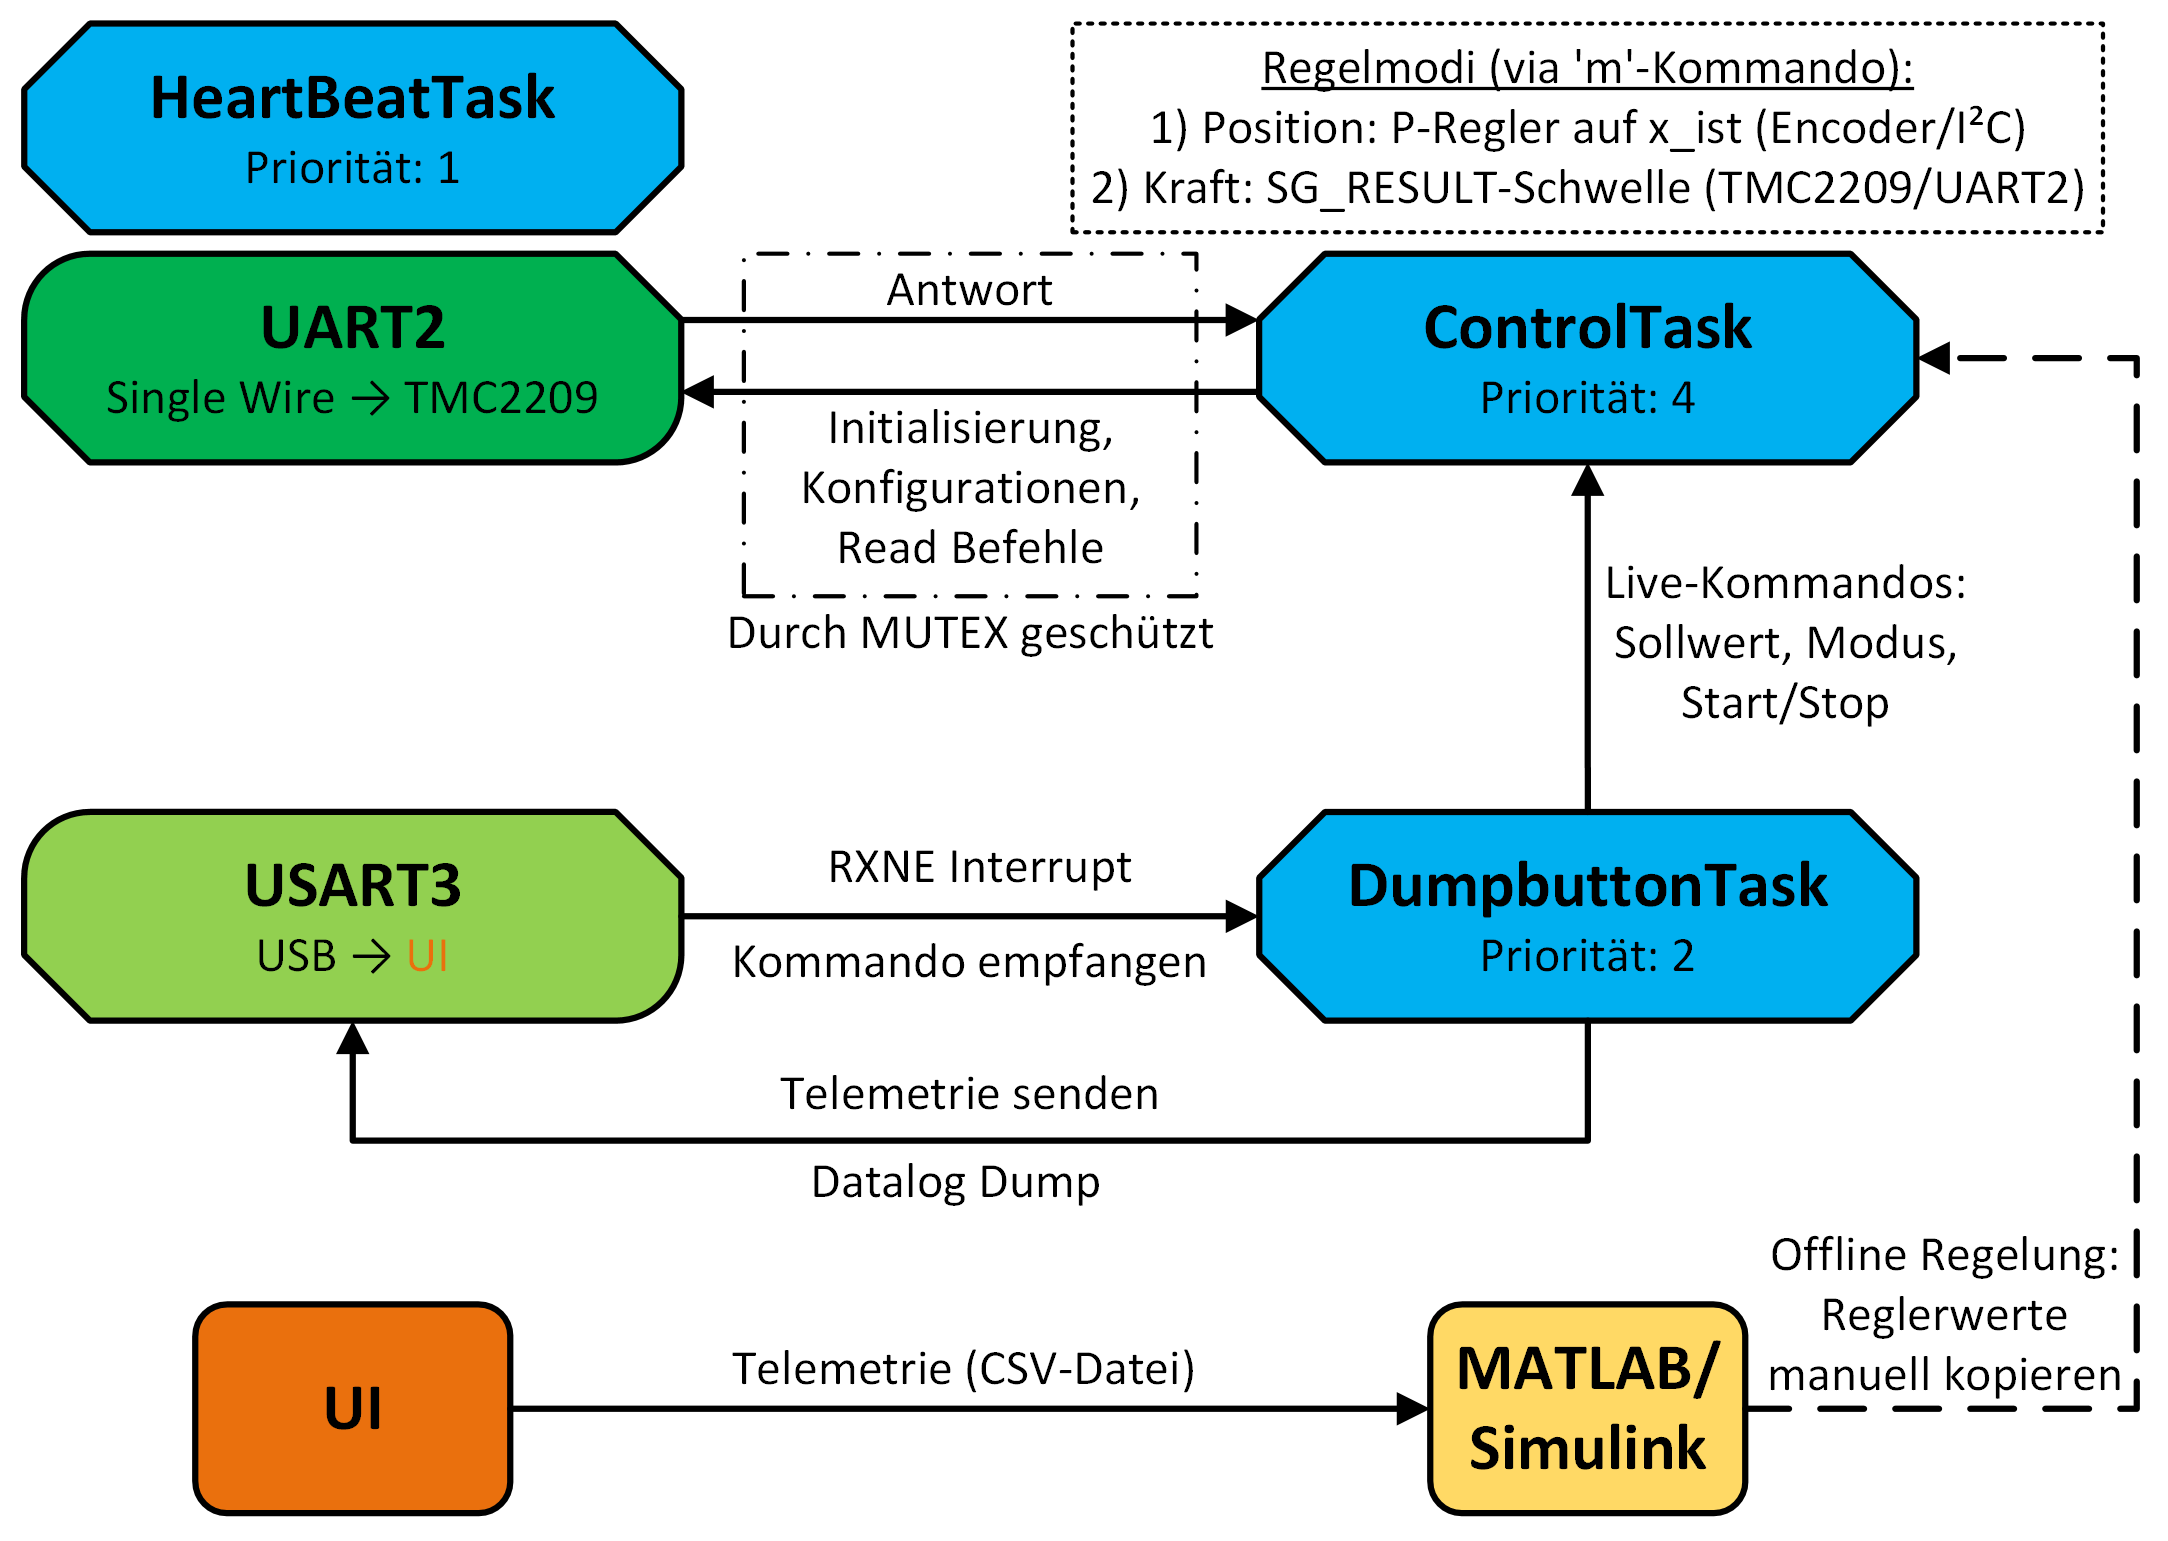
\includegraphics[width=0.85\linewidth]{Abbildung/Programmablauf.png}
    \caption{Grober Programmablauf}
    \label{fig:Programmablauf}
\end{figure}

Den höchstpriorisierten Task (Priorität~4) bildet der \textit{ControlTask}, der in einem festen 2\,ms-Zyklus die eigentliche Regelung ausführt. Er durchläuft einen Zustandsautomaten (\texttt{ST\_ZERO} $\rightarrow$ \texttt{ST\_DIRDETECT} $\rightarrow$ \texttt{ST\_CONTROL} $\rightarrow$ \texttt{ST\_HOLD}/\texttt{ST\_OPEN}/\texttt{ST\_FAULT}) und kann innerhalb des Regelzustands zwischen zwei Reglermodi umschalten, die über ein per USART3 empfangenes \texttt{m}-Kommando ausgewählt werden:

\begin{itemize}
    \item \textbf{Positionsregelung}: Ein P-Regler mit Totzone, Sättigung und Rate-Limiter regelt die Ist-Position (aus dem AS5600-Encoder, I\textsuperscript{2}C) auf einen vorgegebenen Sollwert.
    \item \textbf{Kraft-/Drehmomentregelung}: Auswertung des StallGuard-Werts (\texttt{SG\_RESULT}) des TMC2209-Treibers. Bei Unterschreiten eines vorgegebenen SG-Schwellwerts wird der Vorschub angehalten (indirekte Kraftregelung).
\end{itemize}

Die Kommunikation mit dem Motortreiber erfolgt über \textbf{UART2} als Single-Wire-Verbindung (Halbduplex). Über diese Schnittstelle werden sowohl die einmalige Initialisierung und Konfiguration (Mikroschrittauflösung, Motorstrom) als auch zyklische Lesebefehle (\texttt{SG\_RESULT} für die Kraftregelung) sowie die Geschwindigkeitsvorgaben (\texttt{VACTUAL}) abgewickelt. Da UART2 im Halbduplexbetrieb sowohl vom \texttt{ControlTask} als auch potenziell von parallelen Zugriffen genutzt werden könnte, ist jede Transaktion durch einen Mutex abgesichert.

Der zweite Task, \textit{DumpButtonTask} (Priorität~2), übernimmt die Kommunikation mit der Bedienoberfläche (UI) über \textbf{USART3} (USB-Verbindung). Eingehende Bytes werden zunächst per RXNE-Interrupt in einen Ringpuffer geschrieben. Der Task selbst pollt diesen Puffer alle 20\,ms, parst empfangene Kommandozeilen und setzt daraus globale Zustandsvariablen für Sollwert, Reglermodus und Start-/Stopp-/Öffnen-Befehle. Diese Variablen werden vom \textit{ControlTask} in jedem Regelzyklus ausgelesen und bilden damit den zentralen Steuerkanal zwischen UI und Regelung. Umgekehrt sendet der \textit{DumpButtonTask} periodisch einen Telemetrie-Datensatz sowie einen vollständigen CSV-Dump des Ringpuffer-Datenloggers über dieselbe Schnittstelle an die UI.

Der dritte Task, \textit{}{HeartBeatTask} (Priorität~1), blinkt eine LED im 1\,Hz-Takt und dient lediglich dem Nachweis, dass der Scheduler läuft.

Die von der UI empfangenen Telemetriedaten (CSV-Datei) werden außerhalb der Firmware in MATLAB/Simulink zur Reglerauslegung und -analyse weiterverarbeitet. Die ermittelten Parameter werden manuell als Konstanten in den Quellcode des \textit{ControlTask} übernommen.




% +++++++++++++++++++++++++++++++++++++++++++++++++++++++++++++++++
% Konfiguration von FreeRTOS
% +++++++++++++++++++++++++++++++++++++++++++++++++++++++++++++++++
\section{Konfiguration der MCU und von FreeRTOS}
Die Konfiguration des NUCLEO-F767ZI-Boards wurde in der Entwicklungsumgebung STM32CubeIDE mit dem Firmware Package \textit{STM32Cube FW\_F7 V1.17.3} wie folgt vorgenommen. Nicht explizit genannte Konfigurationen entsprechen den Standardeinstellungen der STM32CubeIDE:

\begin{itemize}
    \item Input Frequenz bei 8 MHz über die HSE und HCLK bei 216 MHz.
    
    \item Timer
    \begin{itemize}
        \item TIM8 als Timebase Source.
        \item TIM3 für Motorbewegungen mit einem Prescaler von 107, sodass unter Betrachtung der APB1 Clock (108 MHz) ein Zähltakt von 1 MHz vorliegt (eine Mikrosekunde pro Tick). TIM3 global interrupt aktiviert.
        \item TIM2 als freilaufender, vom Debugger unabhängiger 32-Bit-Zähler (ein Zählerstand entspricht einer Mikrosekunde) dient als Zeitbasis bzw. liefert Zeitstempel für das Loggen einer Regelabtastung.
    \end{itemize}
    \item USART
    \begin{itemize}
        \item USART2 mit einer Baudrate von 115200 und in der Mode Single Wire (Half Duplex). Pin PD5 wird ohne Pull initialiert.
        \item USART3 mit einer Baudrate von 500000, in Tx\_Rx-Mode und USART3\_IRQn aktiviert. Die Pins PD8 und PD9 werden ohne Pull initialisiert.
    \end{itemize}
    \item GPIO
    \begin{itemize}
        \item Pin PB0 als Output mit User Label \textit{LED\_GREEN}.
        \item Pin PE9 als Output mit Maximum Output Speed auf High und User Label \textit{TMC\_STEP}.
        \item Pin PE11 als Output mit User Label \textit{TMC\_DIR}.
        \item Pin PE13 als Output mit User Label \textit{TMC\_EN}.
    \end{itemize}
    \item GPIO I2C
    \begin{itemize}
        \item Pin PB8 als I2C1\_SCL Signal ohne Pull.
        \item Pin PB9 als I2C1\_SDA Signal ohne Pull.
    \end{itemize}
    \item GPIO NVIC: EXTI line[15:10] interrupts aktiviert.
    \item FreeRTOS Interface Version \textit{CMSIS\_V1}
    \begin{itemize}
        \item USE\_IDLE\_HOOK aktiviert.
        \item USE\_NEWLIB\_REENTRANT aktiviert.
    \end{itemize}
    
\end{itemize}


% +++++++++++++++++++++++++++++++++++++++++++++++++++++++++++++++++
% Motorsteuerung
% +++++++++++++++++++++++++++++++++++++++++++++++++++++++++++++++++
\section{Motorsteuerung}

Die Ansteuerung des Schrittmotors gliedert sich in zwei Softwareebenen: einen registerorientierten UART-Treiber für den Motortreiber TMC2209 (\texttt{tmc2209.h}/\texttt{tmc2209.c}) und eine darüberliegende Motor-Control-Schicht (\texttt{motor\_control.h}/\texttt{motor\_control.c}), die diesen Treiber initialisiert und zusätzliche Bewegungsoptionen bereitstellt.

\subsection{TMC2209-UART-Treiber}

Der TMC2209 wird ausschließlich über die Single-Wire-UART-Schnittstelle  parametriert und angesteuert. Die STEP/DIR-Pins des Treibers selbst kommen nicht zum Einsatz. Das Datagrammformat folgt dem Treiber-Datenblatt: Schreibzugriffe bestehen aus Sync-Byte, Slave-Adresse, Registeradresse (Bit~7 gesetzt) sowie 4 Datenbytes und einem CRC8-Prüfbyte. Lesezugriffe senden eine 4-Byte-Anfrage und erhalten eine 8-Byte-Antwort mit demselben Rahmenaufbau. Die CRC-Berechnung ist in der Funktion \texttt{tmc\_crc()} implementiert und wird sowohl beim Senden als auch beim Validieren empfangener Rahmen verwendet.

Da die Verbindung halbduplex betrieben wird, muss der UART-Treiber vor jedem Lesevorgang explizit vom Sende- in den Empfangsmodus umgeschaltet werden (\texttt{HAL\_HalfDuplex\_ EnableTransmitter}/\texttt{-EnableReceiver}). Gekapselt wird dieser Ablauf durch \texttt{TMC2209\_ Write()} und \texttt{TMC2209\_Read()}: Die beiden Funktionen sichern die gesamte Transaktion – Senden und Empfangen – über einen gemeinsamen Mutex (\texttt{drv->mutex}) ab, sodass parallele Zugriffe verschiedener Tasks auf denselben Bus nicht ineinandergreifen können. Ein Lesevorgang, der den Mutex nicht binnen 50\,ms erhält, wird mit \texttt{false} quittiert anstatt zu blockieren.

Auf dieser Transportschicht setzen mehrere Konfigurations- und Steuerfunktionen auf:
\begin{itemize}
    \item \texttt{TMC2209\_Init()} aktiviert per \texttt{GCONF}-Register die UART-Steuerung (\texttt{pdn\_disable}, \texttt{mstep\_reg\_select}), löscht latente Fehlerflags (\texttt{GSTAT}), aktiviert den Chopper (\texttt{CHOPCONF}, \texttt{TOFF=3}) und liest \texttt{GCONF} zur Verifikation zurück. Schlägt der Chip nicht an, meldet die Funktion \texttt{false}.
    \item \texttt{TMC2209\_SetCurrent()} setzt Lauf- und Haltestrom über das \texttt{IHOLD\_IRUN}-Register (je 0–31, entspricht 1/32 bis 32/32 des Skalenendwerts).
    \item \texttt{TMC2209\_SetMicrosteps()} setzt die Mikroschrittauflösung über das \texttt{MRES}-Feld in \texttt{CHOPCONF} (256 bis 1 Mikroschritte je Vollschritt).
    \item \texttt{TMC2209\_SetStallguardThreshold()} und \texttt{TMC2209\_SeCoolStepThreshold ()} konfigurieren StallGuard4 (\texttt{SGTHRS}) bzw. dessen Gültigkeitsfenster (\texttt{TCOOLTHRS}). Beide Werte bilden die Grundlage für die im \texttt{ControlTask} realisierte StallGuard-basierte Kraftregelung.
    \item \texttt{TMC2209\_MoveVelocity()} schreibt eine Solldrehzahl in das \texttt{VACTUAL}-Register (24 Bit, mit Vorzeichen). In diesem Betriebsmodus erzeugt der TMC2209 die Mikroschritt-Pulse intern. Der Microcontroller muss keine STEP-Flanken mehr ausgeben. \texttt{TMC2209\_Stop()} setzt \texttt{VACTUAL} auf 0.
\end{itemize}

\subsection{Motor-Control-Schicht}

Die Datei \texttt{motor\_control.c} bündelt die Inbetriebnahme des Treibers und stellt zwei alternative Mechanismen zur Bewegungserzeugung bereit, die im Code parallel existieren, aber unterschiedlich stark genutzt werden.

Die Funktion \texttt{MotorControl\_Init()} ruft \texttt{TMC2209\_Init()} in einer Retry-Schleife auf (Wiederholung alle 500\,ms bis zur erfolgreichen Antwort), setzt anschließend feste Betriebsparameter (16 Mikroschritte, \texttt{IRUN=IHOLD=27} für ca.\ 0{,}86\,A\textsubscript{RMS} bei $R_\text{sense}=0{,}11\,\Omega$, ein konservatives StallGuard/CoolStep-Fenster) und aktiviert den Treiber über den Enable-Pin. Über \texttt{MotorControl\_GetDriver()} erhalten andere Module (insbesondere der \texttt{ControlTask}) Zugriff auf den initialisierten TMC2209-Handle, um darüber \texttt{TMC2209\_MoveVelocity()} bzw.\ \texttt{TMC2209\_Read()} (StallGuard) direkt aufzurufen. Durch diesen UART/VACTUAL-Pfad kann der geschlossene Regelkreis im \textit{ControlTask} über \texttt{TMC2209\_MoveVelocity()} kommandiert werden.


% +++++++++++++++++++++++++++++++++++++++++++++++++++++++++++++++++
% Taskeinbindung der Regler
% +++++++++++++++++++++++++++++++++++++++++++++++++++++++++++++++++
\section{Einbindung der Regler in die Taskstruktur}
\label{sec:taskeinbindung}
\textit{Bearbeitet von Mohammad Badr Eddin}\\
Die Firmware basiert auf FreeRTOS. Beide in Kapitel \ref{Kap:Regler}
beschriebenen Regler laufen gemeinsam im zyklischen
\texttt{ControlTask}. Sie verwenden dieselbe Messgröße des AS5600 über
I\textsuperscript{2}C und dieselbe Stellgröße über \texttt{VACTUAL}.
Da immer nur ein Regler aktiv ist, ist eine Aufteilung auf getrennte
Tasks nicht erforderlich.

Der \texttt{ControlTask} besitzt die höchste Priorität aller Tasks.
Sein Regelzyklus wird über eine absolute Zeitbasis auf
\SI{2}{\milli\second} festgelegt. Dadurch bleibt der zeitliche Abstand
zwischen den einzelnen Zyklen unabhängig von der Laufzeit des
Taskrumpfs konstant. Der Zeitstempel für die Messdaten wird direkt
nach dem Aufwecken des Tasks erfasst.

Innerhalb eines Zyklus werden die folgenden Schritte durchlaufen:

\begin{enumerate}
    \item Zeitstempel erfassen,
    \item Encoderwert über I\textsuperscript{2}C lesen und zur
          Istposition verarbeiten,
    \item Treiberstatus über die UART auslesen,
    \item Bedienkommandos und Sollwerte übernehmen,
    \item Zustandsautomat und aktiven Regler ausführen,
    \item Stellgröße als Sollgeschwindigkeit an den Treiber senden,
    \item Messwerte im Ringpuffer speichern.
\end{enumerate}

Die Auswahl des Positions- oder Effort-Reglers richtet sich nach der
aktuellen Betriebsart. Pro Zyklus berechnet nur einer der beiden
Regler die Stellgröße. Die gemeinsame Encoderauswertung,
Stellgrößenbegrenzung und Messdatenspeicherung werden unabhängig von
der Betriebsart nur einmal ausgeführt.

Der Regelzyklus selbst enthält keine Datenausgabe. Die Messwerte
werden zunächst in einem Ringpuffer im Arbeitsspeicher gespeichert
und anschließend von einem niederpriorisierten Task über USART3
übertragen. Sollwerte und Bedienkommandos werden ebenfalls außerhalb
des Regelzyklus in gemeinsamen Variablen hinterlegt. Der
\texttt{ControlTask} übernimmt diese Werte an einer festgelegten
Stelle innerhalb seines Zyklus, sodass die laufende Berechnung nicht
unterbrochen wird.

Die Initialisierung des Motortreibers erfolgt am Anfang des
\texttt{ControlTask}, da sie blockierende UART-Transaktionen enthält.
Während dieser Phase bleibt die Endstufe über das Enable-Signal
abgeschaltet. Die UART-Zugriffe auf den Treiber werden über einen
Mutex geschützt, sodass gleichzeitige Transaktionen nicht
miteinander kollidieren.
% +++++++++++++++++++++++++++++++++++++++++++++++++++++++++++++++++
% Schutz
% +++++++++++++++++++++++++++++++++++++++++++++++++++++++++++++++++
\section{Überlast- und Kollisionsschutz}
\textit{Bearbeitet von Mohammad Badr Eddin}\\

Der Schrittmotor wird im Betrieb über vorgegebene Schrittimpulse
angesteuert. Kommt es zu einer mechanischen Blockade oder einer
Kollision der Greiferbacken, können weiterhin Schrittimpulse erzeugt
werden, obwohl sich der Antrieb nicht mehr bewegt. Eine solche
Situation wird über das Positionsfeedback des AS5600 erkannt. Die
gemessene Bewegung wird mit der vorgegebenen Bewegung des Antriebs
verglichen. Die bestehende Task- und Zustandsautomatenstruktur mit
einer Zykluszeit von \SI{2}{\milli\second} bleibt unverändert.

Für die Erkennung einer Blockade wird nicht nur die aktuelle
Positionsabweichung betrachtet. Während einer normalen Bewegung kann
diese ebenfalls auftreten und würde sonst zu einer fehlerhaften
Abschaltung führen.

Stattdessen wird der Positionsfortschritt über ein Zeitfenster von
\SI{0.15}{\second}, entsprechend 75 Regelzyklen, ausgewertet. Eine
Prüfung erfolgt nur, wenn während mindestens 80\,\% des Zeitfensters
eine ausreichende Bewegungsanforderung vorliegt. Die dafür festgelegte
Mindestgeschwindigkeit beträgt \SI{3}{\milli\meter\per\second}.

Bleibt der gemessene Positionsfortschritt innerhalb eines Zeitfensters
unter \SI{0.2}{\milli\meter}, wird dieses als fehlerhaft bewertet.
Erst drei aufeinanderfolgende fehlerhafte Fenster führen zur
Erkennung einer Blockade bzw. eines möglichen
Schrittverlusts. Die Überwachungsdauer beträgt somit insgesamt
\SI{0.45}{\second}.

Die zeitliche Auswertung verhindert, dass kurze Abweichungen während
der Beschleunigungs- und Bremsphasen oder bei einer Änderung des
Sollwerts unmittelbar eine Abschaltung auslösen.

Wird eine Blockade erkannt, beendet die Steuerung den regulären
Regelbetrieb und wechselt in den Zustand \texttt{ST\_FAULT}. Der Motor
wird über die vorhandene Stopp-Funktion des Treibers angehalten. Im
Fehlerzustand ist die Motoransteuerung durch die Positions- und
Effort-Regelung gesperrt, sodass der Antrieb nicht selbstständig wieder
starten kann. Eine erneute Inbetriebnahme erfolgt erst nach einem
bewussten Neustart der Steuerung. Nach dem Neustart werden die
Initialisierung und die Richtungserkennung erneut durchgeführt.

% % +++++++++++++++++++++++++++++++++++++++++++++++++++++++++++++++++
% % Benutzeroberfläche
% % +++++++++++++++++++++++++++++++++++++++++++++++++++++++++++++++++
% \section{Benutzeroberfläche}
% \textit{Bearbeitet von Masoud Fahim}\\

% [\textit{Umsetzung der UI u.a. zum Umschalten des Reglers}]


